%----------------------------------------------------------
% Rapportmall Martin Isaksson, F02
% http://isaksson.mine.nu:4380/
%
% Inspiration från www.dd.chalmers.se
%
% Jag rekommenderar att läsa "The not so short introduction
% to LaTeX 2e", samt övrig info på www.dd.chalmers.se/latex
%
%----------------------------------------------------------

%----------------------------------------------------------
% Nytt dokument
%----------------------------------------------------------

% A4-papper, textstorlek 10 pt, tvåsidig rapport
\documentclass{tex/martin}

%----------------------------------------------------------
% Paket som används:
%----------------------------------------------------------

\usepackage{fontspec}

%\usepackage{ichiswedish}  % Accept european-encoded (latin1) characters
\usepackage{latexsym}          % Symboler
\usepackage{amssymb}
\usepackage[fleqn]{amsmath}           % Subekvationer (fleqn ger ekvationer vid ett fast avstånd från kanten)
\usepackage{eurosym}           % \euro, \EUR{10} http://www.theiling.de/eurosym.html
\usepackage{graphicx}   % För EPS-figurer
\usepackage{subfig}
\usepackage{moreverb}          % Verbatiminput
\usepackage{fancyhdr}          % Snygga sidhuvuden och sidfötter, se nedan
\usepackage{textfit}           % RIKTIGT stora bokstäver
\usepackage{multicol}          % Kolumner
\usepackage{tabls}             % Större mellanrum i tabeller \\[.3 cm] kan användas också.
\usepackage[swedish]{babel}    % Svenska rubriker i t.ex. innehållsförteckningen
\usepackage{textcomp}          % \textcelsius, \textangle (Euro)
%\usepackage{rotating}         % Roterar text
%\usepackage{a4wide}          % Smala marginaler
%\usepackage{colortbl}          % Färger i tabeller
\usepackage{booktabs}          % Snyggare tabeller
\usepackage{enumerate}   % Snyggare listor: \begin{enumerate}[{Uppg.} a)]
\usepackage{qtree}          % Träd
%\frenchspacing              % Inget extra avstånd efter punkt.

\usepackage{epigraph}    % Coola kapitel
\usepackage{epipart}    % Coola delar (behöver epigraph)
\usepackage{fancyvrb}
\usepackage{lipsum}
\usepackage{color}
\usepackage[usenames,dvipsnames,svgnames,table]{xcolor}

\usepackage{hyperref}  % backref linktocpage pagebackref

\hypersetup{
    %draft, % Uncomment to remove all links (useful for printing in black and white)
    colorlinks=true, breaklinks=true, bookmarks=true,bookmarksnumbered,
    urlcolor=gray, linkcolor=blue, citecolor=green, % Link colors
    pdftitle={}, % PDF title
    pdfauthor={}, % PDF Author
    pdfsubject={}, % PDF Subject
    pdfkeywords={}, % PDF Keywords
    pdfcreator={pdfLaTeX}, % PDF Creator
    pdfproducer={LaTeX with hyperref} % PDF producer
}


\usepackage{caption}
\captionsetup{font=small}
\usepackage{scrhack}
\PassOptionsToPackage{eulerchapternumbers,listings,drafting, pdfspacing, subfig,beramono,eulermath,parts}{classicthesis}
%\usepackage{classicthesis}
%----------------------------------------------------------
% Figurtexter
%----------------------------------------------------------

% DD säger caption2 men det säger inte CTAN.

% Indentering: hang, center, centerlast, nooneline
% Storlek: scriptsize, small, normalsize, large, Large
% Stil: up, it, sl, sc, md, bf, rm, sf, tt

%\usepackage[font=small,labelfont=bf,textfont=it]{mycaption}

%---------------------------------------------------------
% Kapitel
% http://www.ctan.org/tex-archive/macros/latex/contrib/fncychap/
%---------------------------------------------------------

%\usepackage[Lenny]{fncychap}

%---------------------------------------------------------
% Ställ in varje sidas sidhuvud och sidfot.
%---------------------------------------------------------

\fancyhf{}

\renewcommand{\sectionmark}[1]{\markright{\thesection.\ #1}}
\renewcommand{\subsectionmark}[1]{\markright{\thesubsection.\ #1}}

\renewcommand{\headrulewidth}{0pt}  % 0.3pt linje
\renewcommand{\footrulewidth}{0pt}   % 0.3pt linje

%Sidhuvud
\fancyhead[RO]{\thepage}   % Right Odd
\fancyhead[LE]{\footnotesize\rightmark} % Left Even
\fancyhead[RO]{\footnotesize\rightmark}

%Sidfot
\fancyfoot[LE,RO]{\thepage}
\fancyfoot[LO]{\small{Martin Isaksson\newline\emph{martisak@student.chalmers.se}}}
\fancyfoot[RE]{\small{\emph{http://www.dd.chalmers.se/$\sim$martisak}}}

\pagestyle{empty}

%---------------------------------------------------------
% Titelsidan
%---------------------------------------------------------

\begin{document}
\begin{titlepage}

\rubrik{RAPPORTMALL I FYSIK}{för civilingenjörsutbildningen vid}{Chalmers tekniska högskola}

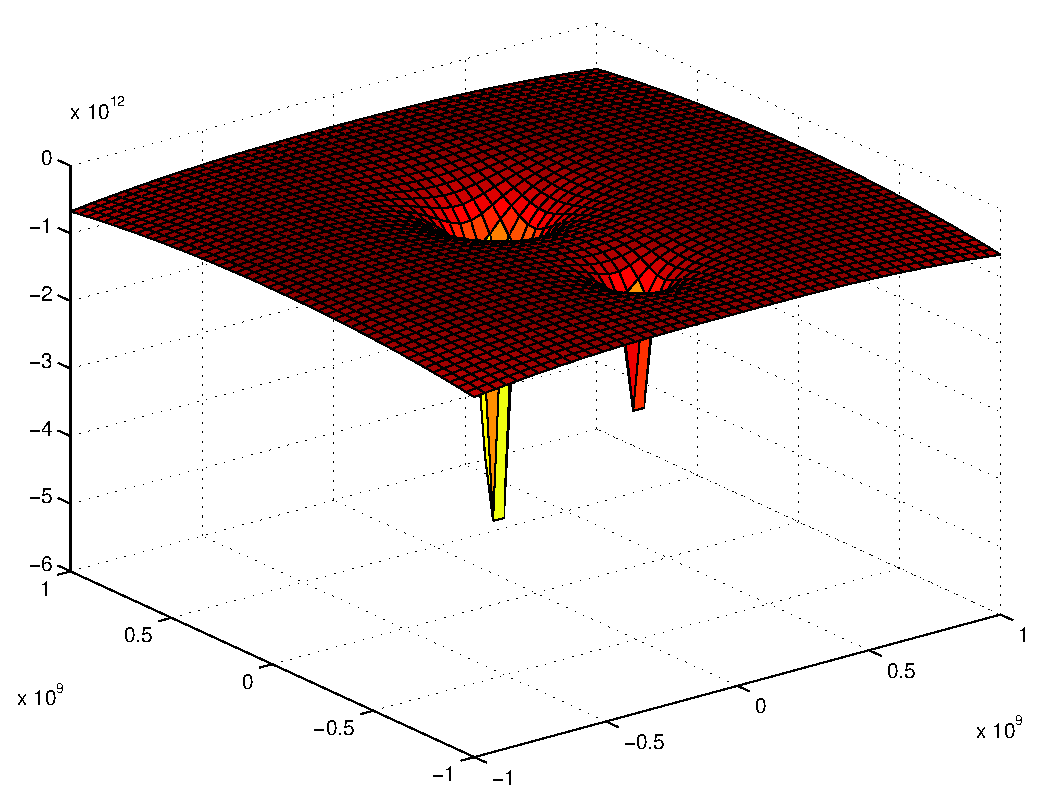
\includegraphics[width=.8\linewidth]{images/surf.eps}   % Lägg till en tuff bild
\vfill                                    % Fyll ut vertikalt

\student{Martin Isaksson}{martisak@student.chalmers.se} % Student 1
% \student{John Doe}{doe@student.chalmers.se}  % Student 2

\vspace{1 cm}
%\small{\emph{Handledare:} Satan}
%\vspace{1 cm}

\small{Chalmers tekniska högskola}   % Skola, ort, etc

\small{\today}                           % Datum

\end{center}
\end{titlepage}

%---------------------------------------------------------
% Sammanfattning.
%--------------------------------------------------------

\cleardoublepage

\begin{center}
\sffamily\textbf{Sammanfattning} \index{Sammanfattning}
\end{center}
Lorem ipsum dolor sit amet, consectetuer adipiscing elit. Aliquam adipiscing gravida odio. Donec non ipsum non tellus egestas tincidunt. In ullamcorper. Phasellus massa eros, malesuada vel, auctor mattis, lobortis nec, quam. Mauris vel lacus. Mauris volutpat ante nec nibh. Donec faucibus varius lorem. Maecenas rhoncus volutpat tortor. Sed nunc. Nam est risus, facilisis a, sollicitudin ut, pretium eu, lectus. Donec scelerisque mi at mi. Cras adipiscing. Pellentesque habitant morbi tristique senectus et netus et malesuada fames ac turpis egestas. Quisque risus. Etiam justo risus, tincidunt ac, faucibus ut, convallis id, pede. Praesent non ligula sit amet augue lobortis cursus.

\vspace{1 cm}

\begin{center}
\sffamily\textbf{Abstract} \index{Abstract}
\end{center}
Lorem ipsum dolor sit amet, consectetuer adipiscing elit. Aliquam adipiscing gravida odio. Donec non ipsum non tellus egestas tincidunt. In ullamcorper. Phasellus massa eros, malesuada vel, auctor mattis, lobortis nec, quam. Mauris vel lacus. Mauris volutpat ante nec nibh. Donec faucibus varius lorem. Maecenas rhoncus volutpat tortor. Sed nunc. Nam est risus, facilisis a, sollicitudin ut, pretium eu, lectus. Donec scelerisque mi at mi. Cras adipiscing. Pellentesque habitant morbi tristique senectus et netus et malesuada fames ac turpis egestas. Quisque risus. Etiam justo risus, tincidunt ac, faucibus ut, convallis id, pede. Praesent non ligula sit amet augue lobortis cursus.

%--------------------------------------------------------
% Innehållsförteckning
%--------------------------------------------------------

\setcounter{tocdepth}{3}   % Antal nivåer i innehållsförteckningen
\pagenumbering{roman}
\cleardoublepage

\setcounter{page}{1}
\tableofcontents % Kompilera alltid två gånger

\addcontentsline{toc}{section}{Figurer}
\listoffigures

\addcontentsline{toc}{section}{Tabeller}
\listoftables

%--------------------------------------------------------
% Indrag
%--------------------------------------------------------

\setlength{\parskip}{12pt}      % Hopp mellan stycken
\setlength{\parindent}{0pt}     % Indrag
\setlength{\mathindent}{24pt}
%--------------------------------------------------------
% Numrering
%--------------------------------------------------------
\renewcommand{\thesection}{\arabic{section}}

\cleardoublepage
\pagenumbering{arabic}
\setcounter{page}{1}     % Se till att detta är sida 1.

%--------------------------------------------------------
% Huvuddokumentet
%--------------------------------------------------------
\pagestyle{plain}

%\chapter{Rapportmall}     % Kapitel, se ovan.

%\chapter{The Social Life of Rabbits}
%\epigraph{Oh! My ears and whiskers!}{Lewis Carroll}

\cleardoublepage\epigraphhead[600]{\emph{``Actl labores jucundi''}}
\part{Inledning}

\cleardoublepage\section{Rapportmall}
\label{sec:rapportmall}

\subsection{Inledning}
\label{subsec:inledning}

Detta är en rapportmall med diverse exempel. Den är ständigt under
utveckling. Om du vet att du kan göra bättre - gör det och visa mig
sedan, målet med mallen är nämligen att lära mig \LaTeX. Jag hoppas
givetvis också att jag i processen lyckas skapa en rapportmall som
fungerar, ser bra ut i allas ögon och ger mig makt och status.

Information om vad den ska \emph{innehålla} finner du på \url{http://www.fy.chalmers.se/edu/lab/pdf/rapportskrivning.pdf}

Nedan infogar jag en riktig slask-text, så att du kan se exempel på
hur man löser vissa saker. Om du saknar någonting så skicka ett mail
så ska jag försöka lösa problemet.

Mallen avänder sig av klassen \texttt{report} samt en massa paket. Du
kommer att behöva paketen \texttt{booktabs}, \texttt{qtree},
\texttt{fncychap} samt \texttt{epigraph}. \texttt{booktabs} behövs för
tabellerna. Det ger t.ex. snyggare linjer. \texttt{qtree} skapar fina
träd. \texttt{fncychap} och \texttt{epigraph} används egentligen inte, men om du vill ha
fina kapitel så kan du använda dem.

\subsection{\texttt{martin.cls}}
\label{subsec:paketet}

Detta är mitt eget paket. Det innehåller en del småsaker som kan vara
nyttiga. Många av dessa är direkt hämtade från
\url{http://www.dd.chalmers.se/latex}. Ett par exempel finns nedan.

En fullständig dokumentation av paketet finns inte än.     % Introduktion till rapportmallen

\cleardoublepage\epigraphhead[600]{\emph{``Aliquando et insanire iucundum est''}}
\part{Exempel}

\cleardoublepage%Slask-innehållet i rapportmallen.

\section{Lorem ipsum dolor sit amet...}
\label{sec:loremipsum}

\nyterm{Lorem ipsum dolor sit amet}{Lorem ipsum dolor sit amet, consectetuer adipiscing elit\cite{loremipsum}.}, consectetuer adipiscing elit\cite{loremipsum}. Proin erat urna, condimentum et, sollicitudin eget, tempus quis, purus. Vestibulum a nisl. Nulla aliquet. Vivamus accumsan. Aenean cursus varius tellus. Maecenas nibh purus, lacinia id, auctor ac, sollicitudin et, magna. Donec lorem ipsum, facilisis sed, consequat porttitor, euismod pulvinar, ante. Mauris venenatis diam sed ligula. Proin justo. Quisque congue posuere est. Class aptent taciti sociosqu ad litora torquent per conubia nostra, per inceptos hymenaeos.

\section{Figurer, tabeller och annat}

\subsection{Trädstrukturer}
\label{subsec:trees}

Paketet \texttt{qtree} tillåter att man ritar träd. Paketet är mycket
syntax-känsligt, men det går att göra en del instressanta saker.

\begin{figure}[!htb]
\begin{center}
\Tree[ .\fbox{Roten} [.{En nod} {Ett löv} ] [.b e f g ]  c d ]
\caption{Ett enkelt träd}
\label{fig:tree}
\end{center}
\end{figure}

Man kan med kommandot \texttt{minipage} skapa figurer som ligger
bredvid varandra. \texttt{linewidth} är sidans bred $0.48$ är alltså
$48$ \% av sidans bredd. Notera utropstecknet i \texttt{[!htb]}.

\begin{figure}[!htb]
  \begin{minipage}[htb]{0.48\linewidth}
    \begin{center}
      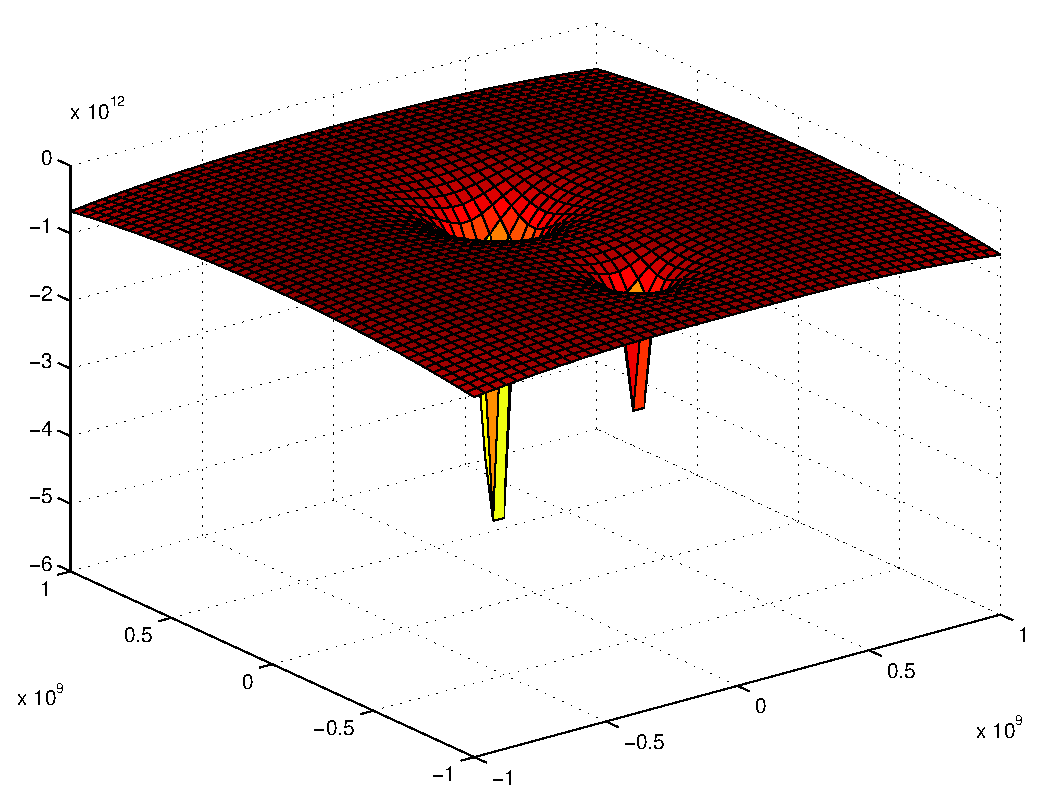
\includegraphics[scale=.35]{images/surf.eps}
    \end{center}
    \caption[Den vänstra figuren.]{Den vänstra figuren är den som är
      till vänster om den högra.}
\label{fig:leftfig}
  \end{minipage}\hfill
  \begin{minipage}[htb]{0.48\linewidth}
    \begin{center}
      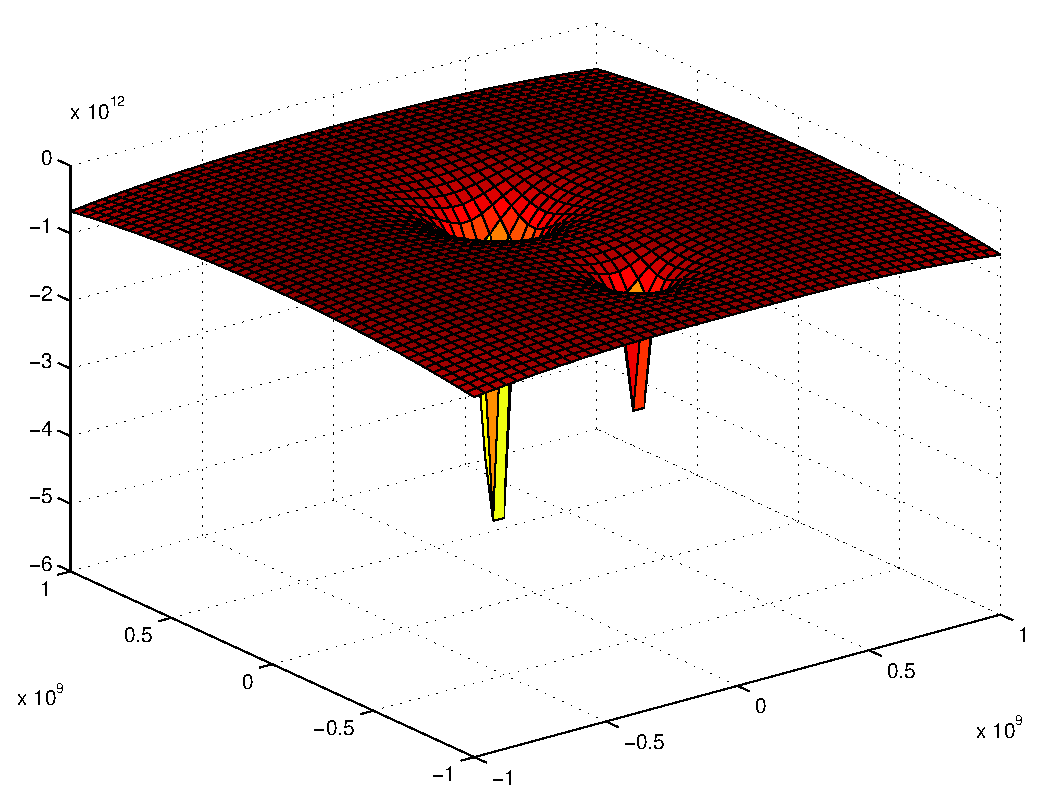
\includegraphics[scale=.35]{images/surf.eps}
    \end{center}
    \caption[Den högra figuren.]{Den högra figuren är den som är
      till höger om den vänstra.}
\label{fig:rightfig}
  \end{minipage}
\end{figure}

\begin{figure}[htb]
  \begin{center}
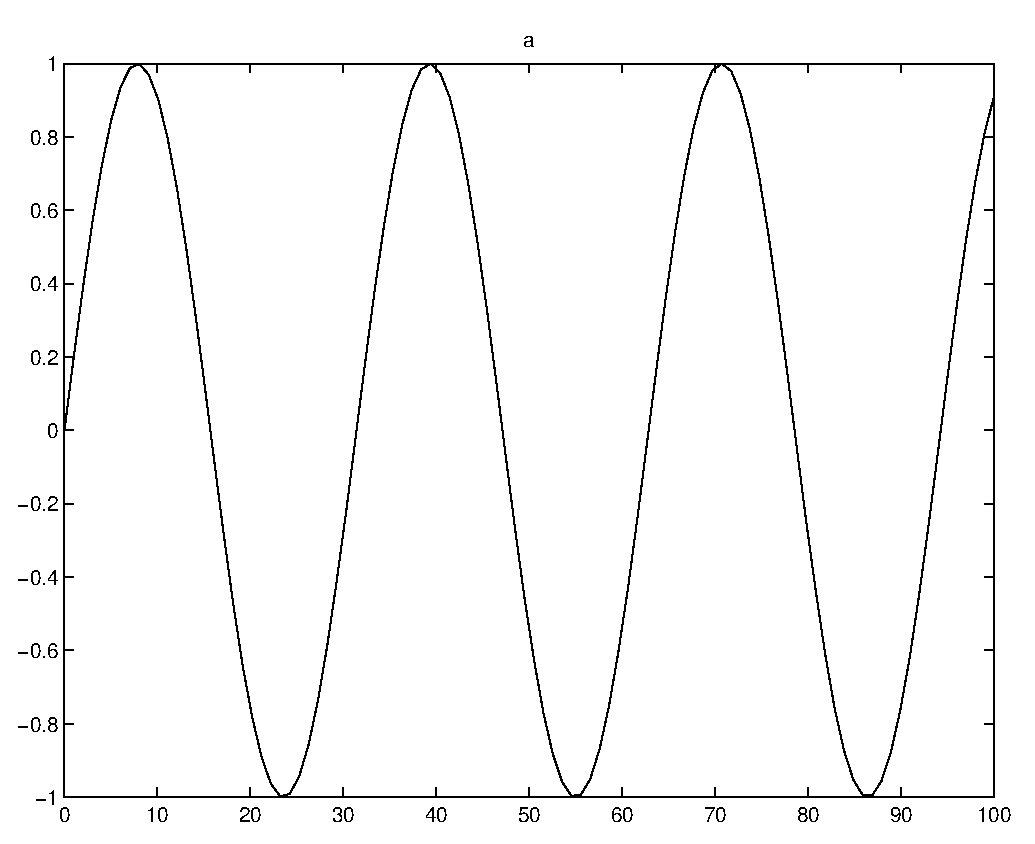
\includegraphics[width=0.8\linewidth]{images/sin.eps}
  \end{center}
  \caption[En ensam figur.]{En ensam figur mitt i sidan.}
\label{fig:center}
\end{figure}

\begin{figure}[!htb]
%\begin{subfigures}
  \begin{minipage}[htb]{0.48\linewidth}
    \begin{center}
      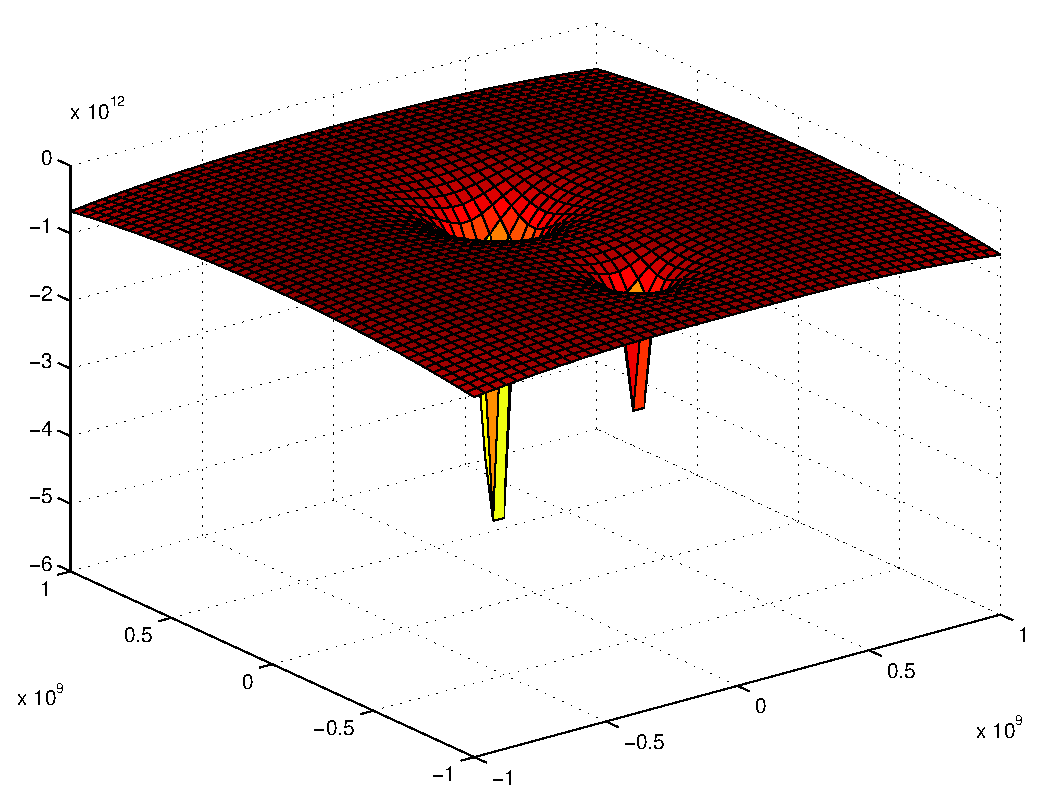
\includegraphics[scale=.35]{images/surf.eps}
    \end{center}
    \caption[Den vänstra figuren.]{Den vänstra figuren är den som är
      till vänster om den högra.}
\label{fig:leftfig2}
  \end{minipage}\hfill
  \begin{minipage}[htb]{0.48\linewidth}
    \begin{center}
      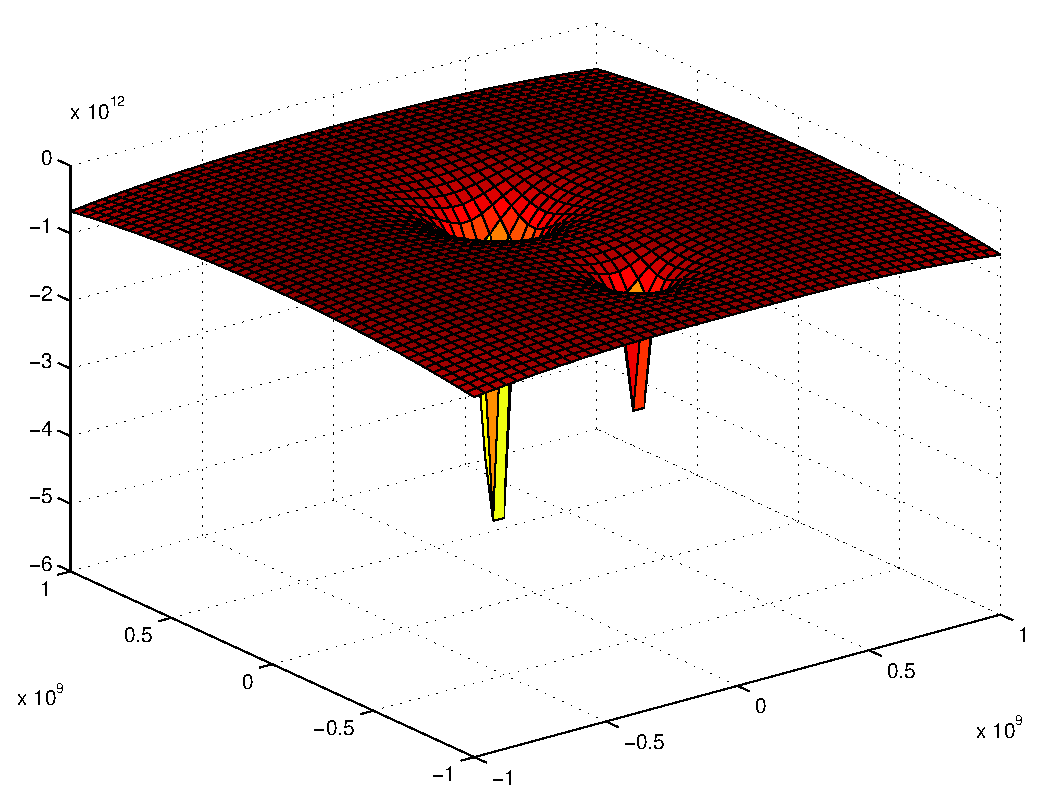
\includegraphics[scale=.35]{images/surf.eps}
    \end{center}
    \caption[Den högra figuren.]{Den högra figuren är den som är
      till höger om den vänstra.}
\label{fig:rightfig2}
  \end{minipage}
%\end{subfigures}
\end{figure}

\subsection{Ekvationer}
\label{subsec:eq}
Ekvationer kan nu ha sub-index.

\begin{subequations}
\begin{align}
a & = b \label{eq:a} \\
c &= d, \label{eq:b}
\end{align}
\end{subequations}

eller vara helt vanliga

\begin{equation}
  \lim_{n \to \infty}2\frac{E_{n+1}-E_{n}}{E_{n+1}+E_{n}}=0.
\label{eq:limn}
\end{equation}
\subsubsection{Spännande saker i ekvationer}
\label{subsubsec:spannend}
\begin{equation}
 A(n)\xrightarrow[n\to\infty]{}0
\end{equation}

\subsection{Tabeller}
\begin{table}
  \begin{center}
  \caption[Energier vid olika kvanttal]{Energier vid olika kvanttal ($1$ H $\approx$ $27.2$ eV)}
    \begin{tabular}{cc}\toprule
      $n$ & $E_n$ [Hartree]\\ \midrule
      $1$ & $1.23$ \\
      $2$ & $4.93$ \\
      $3$ & $11.10$\\
      $4$ & $19.74$\\
      $5$ & $30.84$\\
      $6$ & $44.41$\\
      $7$ & $60.45$\\
      $8$ & $78.96$\\
      $9$ & $99.93$\\
      $10$ &$123.37$\\ \bottomrule
    \end{tabular}

\label{tbl:energy}
  \end{center}
\end{table}

\subsection{Referenser och andra små ting}
\label{subsec:ref}

Man kan referera till ekvationer enligt Ekvation \eqref{eq:a}, till figurer och tabeller enligt Tabell \ref{tbl:energy} och till någon källa så här\cite{lshort}.

\itauthquote{Do you really believe the moon is not there if nobody looks?}{Albert Einstein (citerad av Pasqual Jordan)}

Citat som det ovan är en del av paketet \texttt{martin}.

\section{Kolumner}
\begin{multicols}{2}[\subsection{2 Kolumner}]
Lorem ipsum dolor sit amet, consectetuer adipiscing elit. Aliquam adipiscing gravida odio. Donec non ipsum non tellus egestas tincidunt. In ullamcorper. Phasellus massa eros, malesuada vel,  auctor mattis, lobortis nec, quam. Mauris vel lacus. Mauris volutpat ante nec nibh. Donec faucibus varius lorem. Maecenas rhoncus volutpat tortor. Sed nunc. Nam est risus, facilisis a, sollicitudin ut, pretium eu, lectus. Donec scelerisque mi at mi. Cras adipiscing. Pellentesque habitant morbi tristique senectus et netus et malesuada fames ac turpis egestas. Quisque risus. Etiam justo risus, tincidunt ac, faucibus ut, convallis id, pede. Praesent non ligula sit amet augue lobortis cursus.
\end{multicols}

%\section{Rotating}
%
%\begin{sideways} Lorem ipsum dolor sit amet. \end{sideways}
%\begin{turn}{45} Lorem ipsum dolor sit amet.\end{turn}
%\begin{rotate}{30} Praesent non ligula sit amet augue lobortis cursus.\end{rotate}
%\turnbox{-15}{Praesent non ligula sit amet augue lobortis cursus.}     % Infogar slask-texten.

\cleardoublepage\epigraphhead[600]{\itauthquote{I never guess. It is a capital mistake to theorize before one has data.
Insensibly one begins to twist facts to suit theories, instead of theories to
suit facts.}{Sir Arthur Conan Doyle}}
\part{Rapportmall}

\cleardoublepage% Sj�lva mallen
% Fr�n http://www.fy.chalmers.se/edu/lab/pdf/rapportskrivning.pdf
\section{Introduktion}
\lipsum
\section{Experiment}
\lipsum
\section{Resultat}
\lipsum
\section{Diskussion}
\lipsum
\section{Slutsats}
\lipsum     % Fysik-mallen från http://www.fy.chalmers.se/edu/lab/pdf/rapportskrivning.pdf

%--------------------------------------------------------
% Referenslista
%--------------------------------------------------------

\nocite{*}
\bibliographystyle{plain}
\bibliography{rapportmall}
\thispagestyle{empty}

%--------------------------------------------------------
% Appendix
%--------------------------------------------------------

\bilaga
\section{MATLAB-kod}\label{matlab}
\subsection{Plancks strålningslag}\label{planckslag}
\subsubsection{planck.m}

\renewcommand{\theFancyVerbLine}{\textit{\texttt{\arabic{FancyVerbLine}}}}

%\catcode33=\active

\def\ExclamationPoint{\%}
\catcode33=\active
\def !{\%}

\VerbatimInput[defineactive=\def!{\itshape\ExclamationPoint},numbers=left, numbersep=0.5cm]{code/planck.m}

\end{document}

%--------------------------------------------------------